% \documentclass[12pt]{article}

%%v helpful MIT exam schema, see http://www-math.mit.edu/~psh/exam/examdoc.pdf
 \documentclass[12pt]{exam} 
% \qformat{\textbf{Question \thequestion}\quad \thepoints\hfill } % Large depth to make space}
 \renewcommand{\thesubpart}{(\roman{subpart})}
 \renewcommand{\subpartlabel}{\thesubpart}
 \footer{}{}{Page \thepage\ de \numpages}
\addpoints
\pointsinmargin
% \boxedpoints
\renewcommand{\questionshook}{\setlength{\itemsep}{0.2cm}}
\renewcommand{\partshook}{
	\setlength{\itemsep}{5mm}
}

\usepackage{cmbright}

\pagestyle{empty} %for handouts
\addtolength{\jot}{2em} % this makes all formulae a bit more spaced vertically for handouts
\setlength{\parindent}{0pt} %we're not writing a novel
%\renewcommand{\arraystretch}{2} %makes tables taller, so easier to write in

\usepackage[fleqn]{amsmath}
\usepackage{amssymb} %standard classy maths symbols
\usepackage[a4paper, margin=1in]{geometry} %makes it easy to specify where to put stuff on the page

\usepackage{siunitx} %v handy way of getting SI units to typeset correctly...
% \sisetup{locale = FR} %... and now it will use a comma for decimals

\usepackage[utf8]{inputenc}

% \usepackage[french]{babel} % frenchify everything (e.g. a Table becomes a Tableau)
% \usepackage{lmodern} % font with nicer French characters than standard
% \usepackage{textcomp} % and more help for special characters

\usepackage{tcolorbox} % basic but good package for boxes around text
\tcbset{colback=black!5!white}
% \usepackage{color} % colours
%\newcommand{\fillin}{\color{black!1!white}} %makes the text disappear
%\definecolor{fillin}{rgb} {1.00,1.00,1.00}
%\renewcommand{\fillin}{\color{blue}} \definecolor{fillin}{rgb} {0.00,0.00,1.00} %makes the filling in text appear (in blue)

\usepackage{enumitem} % can change the labels on lists, items, enumerates
\usepackage{setspace}

\usepackage{tikz}

\usepackage{multicol}

\begin{document}

\small

\textbf{Name:} \dotfill

\begin{questions}

\question[6] Simplify the following expressions fully:

\begin{parts}

\begin{multicols}{2}
\part $a^5 \cdot a^2 =$ \dotfill
\part $\left(x^{3}\right)^4 =$ \dotfill
\part $(2y)^3 \cdot y^{-1} = $ \dotfill
\part $\displaystyle 81^{1/4} = $ \dotfill
\end{multicols}

\part $\displaystyle \frac{(x^2y)^3}{x^5y^3} = $ \dotfill
\part $\displaystyle \sqrt[4]{a^2 b^8 \cdot \sqrt{c}} \cdot \sqrt[8]{c^7 d^4} = $ \dotfill

\end{parts}


\question[3] Write the following numbers in scientific notation:
\begin{parts}
\begin{multicols}{2}
\part $320000 =$ \dotfill
\part $0.00000053 =$ \dotfill
\end{multicols}

\part $3000^{702} \cdot 3^{-700} =$ \dotfill
\fillwithdottedlines{12mm}

\end{parts}

\question[4] Fill in the following table of values, to 1 decimal place, and then plot the graph of $y = 2^x$.
\begin{minipage}[t]{0.25\textwidth}
\vspace{0mm}
\[
\begin{array}{|c|c|}
\hline
x & \quad y = 2^x \quad \\[6pt]
\hline
-4 & \\[6pt] \hline
-3 & \\[6pt] \hline
-2 & \\[6pt] \hline
-1 & \\[6pt] \hline
0 & \\[6pt] \hline
1 & \\[6pt] \hline
2 & \\[6pt] \hline
3 & \\[6pt] \hline
4 & \\[6pt] \hline
\end{array}
\] 

\end{minipage}
\hfill
\begin{minipage}[t]{0.55\textwidth}
\vspace{0mm}

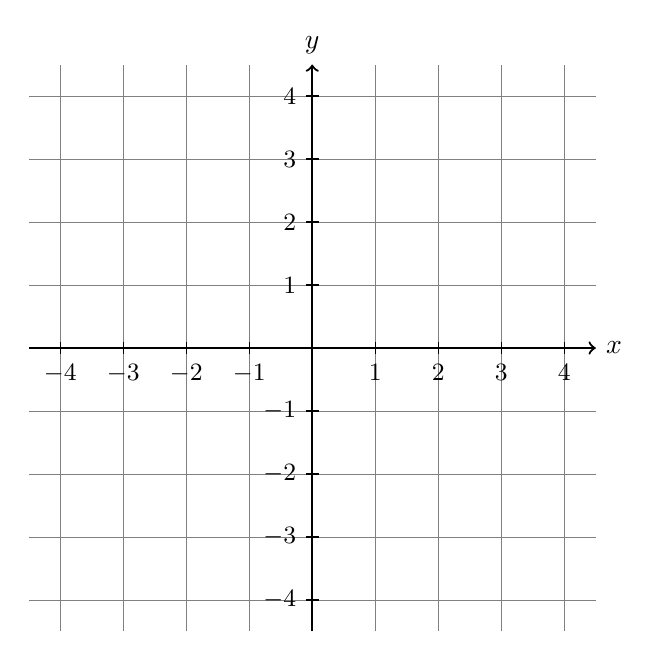
\begin{tikzpicture}[scale=0.8]
    % Draw grid
    \draw[step=1cm,gray,very thin] (-4.5,-4.5) grid (4.5,4.5);

    % Draw axes
    \draw[thick,->] (-4.5,0) -- (4.5,0) node[right] {$x$};
    \draw[thick,->] (0,-4.5) -- (0,4.5) node[above] {$y$};

    % Label axes
    \foreach \x in {-4,-3,-2,-1,1,2,3,4}
      \draw (\x,0.1) -- (\x,-0.1) node[below] {\small $\x$};

    \foreach \y in {-4,-3,-2,-1,1,2,3,4}
      \draw (0.1,\y) -- (-0.1,\y) node[left] {\small $\y$};
\end{tikzpicture}

\end{minipage}

\vfill

\question \textbf{Bonus.} Solve $7^{x+3} = 49^x$. \hfill \emph{Work on the back.}

\end{questions}



\begin{tcolorbox}

\textbf{Name of marker:}

\begin{center}
\gradetable[h][questions]
\end{center}

\end{tcolorbox}

\end{document}